\documentclass[paper=a4, fontsize=12pt]{scrartcl}
\usepackage{graphicx}
\usepackage[protrusion=true,expansion=true]{microtype}
\usepackage{amsmath,amsfonts,amsthm}
\usepackage{fourier}
\usepackage[utf8]{inputenc}
\usepackage{amsmath}
\usepackage{amsfonts}
\usepackage{amssymb}
\usepackage[OT4]{fontenc}
\usepackage[polish]{babel}
\usepackage{epstopdf}
\usepackage{fancyhdr}
\usepackage{hyperref}
\pagestyle{fancyplain}
\fancyhead{}	
\renewcommand{\headrulewidth}{1pt}
\renewcommand{\footrulewidth}{1pt}
\textheight = 700pt
\textwidth = 500pt
\hoffset =-30pt
\begin{document}
\begin{flushright}
17.03.2016 r.\\
dr Robert Bryl
\end{flushright}Paweł Grabiński\\
Rok 3, Fizyka teoretyczna\\[0.5cm]
{\huge \bf Doświadczenie Franka-Hertza}
\section{Wyniki}
Energia wbudzenia dla atomu rtęci wynosi: $E_{ex}=(4.78\pm0.11)\:\mathrm{eV}$
\section{Tabela pomiarowa}
\label{sec:tabpom}
Pomiary\footnote{Dane zostały przedstawione w postaci wykresów i dołączone jako załącznik} przez nas zebrane:

\begin{table}[h]
\begin{center}
	\begin{tabular}{|l|l|l|l|l|}
		\hline
		$T\:[^\circ\mathrm{C}]$ & $U_{1}\:[\mathrm{V}]$ & $U_{2}\:[\mathrm{V}]$ & $U_{12}\:[\mathrm{V}]$ & $U_{res}\:[\mathrm{V}]$ \\ \hline
		67 & 1.95 & 6.8  & 4.85  & 0.5 \\ \hline
		67  & 2.15 & 6.7  & 4.55  & 2.  \\ \hline
		67  & 2.35 & 6.5  & 4.15  & 2.5 \\ \hline
		67  & 2.   & 6.8  & 4.8   & 1.  \\ \hline
		72  & 2.05 & 6.8  & 4.75  & 1.5 \\ \hline
		72  & 2.1  & 6.7  & 4.6   & 2.  \\ \hline
		72  & 2.25 & 6.55 & 4.3   & 2.5 \\ \hline
		72  & 1.85 & 6.8  & 4.95  & 0.5 \\ \hline
		72  & 1.9  & 6.85 & 4.945 & 1.  \\ \hline
		78  & 1.95 & 6.8  & 4.85  & 1.5 \\ \hline
		78  & 1.9  & 6.8  & 4.9   & 1.5 \\ \hline
		78  & 1.8  & 6.8  & 5.    & 0.5 \\ \hline
		78  & 1.85 & 6.85 & 5.    & 1.  \\ \hline
		78  & 1.95 & 6.75 & 4.8   & 2.  \\ \hline
		83  & 2.1  & 6.65 & 4.55  & 2.5 \\ \hline
		83  & 1.75 & 6.8  & 5.05  & 0.5 \\ \hline
		83  & 1.75 & 6.85 & 5.1   & 1.  \\ \hline
		83  & 1.85 & 6.8  & 4.95  & 1.5 \\ \hline
		83  & 1.9  & 6.75 & 4.85  & 2.  \\ \hline
		83  & 2.   & 6.7  & 4.7   & 2.5 \\ \hline
	\end{tabular}
\end{center}
\end{table}

\newpage
\section{Opis teoretyczny}
	
\subsection{Serie widmowe}
Badając widma atomowe zauważono, że są one dyskretne i tworzą linie spektralne. Kolejnym istotnym spostrzeżeniem było, że nie są one położone chaotycznie, lecz układają sie w grupy - serie spektralne. Każda z serii widmowych ma jeden stan kwantowy jako stan końcowy atomu. Dla wodoru Balmer pokazał, że prawdziwa jest zależność:
	\begin{equation}
	\lambda = \lambda_0 - \frac{n^2}{n^2 -4}
	\end{equation}
	Gdzie $\lambda_0$– stała, n – liczba całkowita, przebiegająca znaczenia 3,4,5 itd.
	W spektroskopii najczęściej najczęściej posługujemy się częstotliwością fali:
	\begin{equation*}
	\nu=\frac{c}{\lambda}
	\end{equation*}
Przekształcając wyrażenie $(1)$ otrzymamy:
		\begin{equation}
		\nu= Rc \left(  \frac{1}{2^2} - \frac{1}{n^2}  \right),\qquad n=3,4,5,\dots
		\end{equation}	
Teraz dla dowolnej serii mamy wzór Balmera:
		\begin{equation}
		\nu= Rc \left(  \frac{1}{m^2} - \frac{1}{n^2}  \right),\qquad n=3,4,5,\dots
		\end{equation}
Teraz w zależności od $m$ poszczególne serie nazywamy:
\begin{itemize}
	\item Seria Lymana(ultrafiolet): $m=1$
	\item Seria Balmera: $m=2$
	\item Seria Paschena(podczerwień): $m=3$
	\item Seria Pfunda: $m=4$
	\item Seria Humphreysa: $m=5$
\end{itemize}
Jako komentarz historyczny można dodać, że Balmer nie był fizykiem, a numerologiem. Powyższą prawdiłowość otrzymał na podstawie danych, które otrzymał na znajomego fizyka.

\subsection{Model wektorowy atomu}
Atom rtęci ma $80$ elektronów, w tym $2$ walencyjne. Model wektorowy atomu rtęci zbudowany jest z dwóch par wektorów: orbitalnego momentu pędu $\vec{l_i}$ i spinowego momentu pędu $\vec{s_i}$. Wartości tych wektorów wyrżają się jako :\begin{align*}
|l|=\hbar \sqrt{l(l+1)}, \qquad |s|=\hbar \sqrt{s(s+1)}.
\end{align*}
Ponieważ nie można jednoznacznie zdefiniować wartości wektora w danym kierunku, to posługujemy się rzutami na te kierunki, co umożliwia sumowanie.Całkowity wektor momentu pędu $\vec{J}$ jest stały: \begin{align*}
|J|=\hbar \sqrt{j(j+1)},\qquad j = l+s, l+s-1, ... ,|l-s|.
\end{align*}	
Od liczb kwantowych $l$ i $s$ zależą dyskretne poziomy atomowe i możliwe przejścia z jednego poziomu na drugi. 

\subsection{Diagram Grotriana dla rtęci}
Przedstawienie degeneracji poziomów energetycznych elektronów w atomie. Dozwolone przejścia zanzaczone są liniami. Diagram ma podwójną skalę. Po lewej mamy potencjał wzbudzający wyrażonych w woltach, a po prawej długość fali odpowiadającej fotonowi emitowanemu lub absorbowanemu przy przejściu.
\begin{figure}[h!]
	\begin{center}
	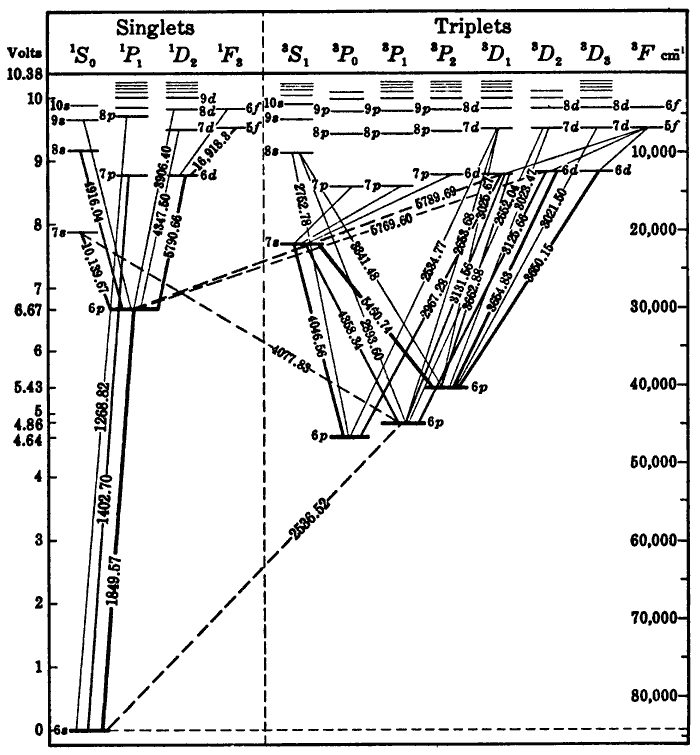
\includegraphics[width=0.65\linewidth]{x.png}\\	\caption{Diagram Grotriana dla Hg}
	\end{center}
\end{figure}
\subsubsection{Zasady wyboru}	
Nie każde przejście elektronu w atomie jest dozwolone. Niektóre wymagają specjalnych zjawisk wymiany, jak na przykład wymiana elektronów o przeciwnych spinach przez atomy w wyniku zderzenia i przejście pomiędzy stanami singletowymi i tripletowymi. Dla atomu rtęci najbardziej możliwym z przejść jest przejście odpowiadające absorobcji lub emisji fotonu o energii $4.9\:\mathrm{eV}$.
\subsection{Linie rezonansowe}
Linia rezonansowa to linia spektralna związana z przejściami elektronu pomiędzy stanem podstawowym i pierwszy stanem wzbudzonym (rezonansowym) z wymianą fotonu $h\nu$. Dla atomu rtęci możemy przedstawić ten proces jako:
		\begin{equation*}
		h\nu=E_n - E_m = 4.9\:\rm{eV}\Rightarrow \lambda =253.5\:\mathrm{nm}= 2535 \:\mathring{\mathrm{A}}
		\end{equation*}
\subsection{Rodzaje zderzeń elektronów z atomem. Efekt Ramsauera, przekrój czynny na zderzenia}	
		
		W zderzeniach elektronu z atomem rozróżniamy zderzenia sprężyste i niesprężyste (I i II rodzaju/0.
\subsubsection{Zderzenia sprężyste}
W zderzeniach sprężystych zachowane są wartości energii i pędu, ale zmieniony jest kierunek ruchu. Zachodzą głównie, gdy elektron ma energię niższą niż energia wzbudzenia atomu.
\subsubsection{Zderzenia niesprężyste}
Zderzenia niesprężyste odbywają się z wymianą energii.
\begin{itemize}
	\item I rodzaju - elektron oddaje swoją energię wzbudzając atom
	\item II rodzaju - atom przechodząc do stanu podstawowego oddaje energię elektronowi
\end{itemize}
		
\subsubsection{Efekt Ramsauera}
Naturalnym jest, że rozpraszając elektrony na atomie oczekujemy, że przekrój czynny maleje z prędkością elektronów. I przeciwnie, oczekujemy, że gdy prędkość maleje, to przekrój czynny będzie wzrastać. Jednak do pewnego momentu, gdy elektrony będą tak niską energię kinetyczną, że nie będzie dochodziło do rozpraszania.
Zjawisko to nazywamy efekt Ramsauera.		
\subsection{Pomiar potencjału wzbudzenia i jonizacji}
Przejściu ze stanu wzbudzonego(rezonansowego) do stanu podstawowego atomu rtęci towarzyszy emisja fotonu o długości fali $\lambda =2535\:\mathrm{\AA}$. Zmierzyć potencjał wzbudzenia atomu rtęci możemy w następująco: do uzyskania promieniowania o wspomnianej długości fali używa się lampy rtęciowej w tak dobranym polu magnetycznym, żeby łuk rtęciowy odginięty przez to pole przebiegał bezpośrednio przy kwarcowej ściance lampy. Za pomocą specjalnego filtru barwnego przepuszczającego tylko fale o długości krótszej niż $3000\:\mathrm{\AA}$ soczewką kwarcową skupiamy światło lampy rtęciowej na tzw. lampie rezonansowej. Para rtęci w kuli znajdującej się za lampą, filtrem i soczewką naświetlona jest światłem monochromatycznym o danej rezonansowej długości, co prowadzi do wzbudzenia atomów pary. Stan wzbudzony nie jest trwały - po $10^{8}\:\mathrm{ s}$ atom przechodzi do stanu podstawowego emitując przy tym foton o tej samej długości fali. Lampa rezonansowa powinna więc wysyłać we wszystkie kierunki promieniowanie, odpowiadające wspomnianemu przejściu, można obserwować na ekranie fluoryzującym. Jeżeli umieścimy pomiędzy lampą a ekranem parę rtęci, to zaobserwujemy na ekranie cień - fotony są absorbowane prze atomy pary. 
		

		
\subsection{Doświadczenie Francka-Hertza}
Układ pomiarowy składa się z:
\begin{itemize}
\item katody będącej źródłem wiązki elektronów (\textbf{Filament}),
\item dwóch siatek, których napięcie możemy kontrolować, służących do rozpędzania elektronów (\textbf{Cathode} i \textbf{Anode(grid)}),
\item anody, zbierającej elektrony, z możliwością pomiaru natężenia prądu (\textbf{Collector}),
\item szklanej komory próżniowej zawierającej naparowaną rtęć.
\end{itemize}
Elektrony generowane przez katodę trafiają do obszaru pomiędzy siatkami, gdzie są przyspieszane przez pole elektryczne. W obszarze tym również znajduje się para rtęci. Elektrony mogą zderzać się z atomami. Gdy osiągną odpowiednią energię, może dojść do zderzenia niesprężystego i przekazania energii od elektornu do atomu. Dalej elektron może być ponownie przyspieszony do odpowiedniej energii i ponownie wzbudzić atom. Po przekroczeniu drugiej siatki, elektrony wpadają w obszar potencjału progowego, do którego pokonania potrzebują odpowiedniej energii.
		\begin{figure}[h!]
			\centering
			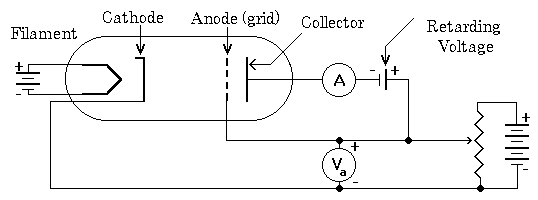
\includegraphics[width=10 cm]{e.png}
			\caption{Układ pomiarowy doświadczenia Franka-Hertza}
		\end{figure}
\subsection{Interpretacja wyników}
\begin{figure}[h!]
\centering
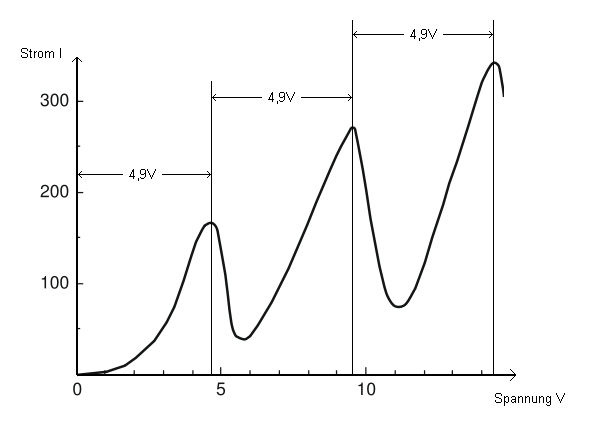
\includegraphics[width=0.5\linewidth]{franck_hertz_02}
\caption{Przykładowy wykres danych zmierzonych w doświadczeniu Francka-Hertza}
\label{fig:franck_hertz_02}
\end{figure}
Widzimy wielokrotne maksima i minima prądu anodowego w zależności od przyłożonego napięcia przyspieszającego. Maksima pojawiają się w okolicach $4.9\:\mathrm{V}$. Jest to sytuacja, gdy elektronom brakuje energii, by wzbudzić atomy rtęci. Natomiast minima odpowiadają napięciom $4.9\:\mathrm{V}+U_{res}$, gdzie elektorny mają energię wystarczającą, by wzbudzić atom, ale niewystarczająca, by pokonać potencjał zaporowy. Isotną obserwacją jest fakt występowania minimów i maksimów co stałą wartość, co dowodzi hipotezy dyskretnych poziomów energetycznych.
\newpage
\section{Opis doświadczenia}
Pierwszą czynnością naszego eksperymentu jest podniesienie temperatury układu do temperatury początkowej $65\:^\circ \mathrm{C}$. Po dojściu układu do równowagi termiczej, możemy przystąpić do pomiarów. Dla każdej badanej temperatury ($T\in\left\lbrace65\:^\circ \mathrm{C},\: 70\:^\circ \mathrm{C},\: 75\:^\circ \mathrm{C},\: 80\:^\circ \mathrm{C}\right\rbrace$), za pomocą układu pomiarowego połączonego z komputerem, mierzymy natężenia prądu anodowego w zależności od napięcia przyspieszającego. Pomiary wykonujemy dla $5$ różnych wartości napięcia progowego $U_{res}\in\left\lbrace0.5\:\mathrm{V},\:1\:\mathrm{V},\:1.5\:\mathrm{V},\:2\:\mathrm{V},\:2.5\:\mathrm{V}\right\rbrace$.
\section{Obliczenia}
Wartości potencjału wzbudzenia atomu rtęci będziemy wyzaczać z różnic pomiędzy kolejnymi maksimami prądu anadowego. Patrząc na wykresy widzimy, że pierwsze oraz drugie maksima zachowują się dobrze niezależnie od pomiaru, jednak dalsze maksima często mają duże zakłócenia lub są nieodróżnialne od szumu. Dlatego liczymy różnice pomiędzy pierwszym i drugimi maksimami dla wszystkich $20$ zestawów danych (wyniki znaleźć można w \textbf{Tabeli Pomiarowej} \ref{sec:tabpom}). Dalej liczymy średnią arytmetyczną tych wyników i dostajemy wynik:
\begin{align*}
U_{ex}=4.7825\:\mathrm{V}
\end{align*}
Czyli energia wbudzenia atomu rtęci, to:
\begin{align}
E_{ex}=4.7825\:\mathrm{eV}
\end{align}
\section{Niepewności pomiarów}
Niepewność pomiarową możemy uzyskać ze wzoru:
\begin{align*}
\Delta U=\frac{U_{max}-U_{min}}{2\sqrt{N}}
\end{align*}
W naszym przypadku wynosi to:
\begin{align*}
\Delta U=\frac{5.1-4.15}{2\sqrt{20}}=0.106213\approx 0.11
\end{align*}
Niepewność naszego pomiaru, to $\Delta U=0.11\:\mathrm{V}$.
\section{Wnioski}
Wartość tabelaryczna energii wzbudzenia dla atomu rtęci to $4.9\:\mathrm{eV}$. \\
W naszych pomiarach otrzymaliśmy $E_{ex}=(4.78\pm0.11)\:\mathrm{eV}$. Widzimy, że jest to wartość bardzo zbliżona.

Jednak sama wartość energii wzbudzenia jest tylko pobocznym wnioskiem doświadczenia. Najistotniejszą obserwacją jest powatarzanie się maksimów, co stałą wartość potencjału przyspieszającego. Do tej obserwacji najlepsze są pomiary przy niskich napięciach oporowych i wysokich temperaturach. Na wykresach odpowiadających tym warunkom możemy zauważyć nawet $4$ wyraźne maksima.

Wyniki stają się mniej czytelne przy dużych napięciach oporowych. By potwierdzić hipotezę dyskretnych poziomów energii najlepiej badać $0.5-1.5\:\mathrm{V}$ potencjału progowego.

Ciekawe zjawisko możemy zauważyć przy dużych temperaturach oraz dużych napięciach oporowych. Gdy przyłożymy duże napięcie przyspieszające, prąd anadowy zmienia kierunek i płynie w drugą stronę. Z powodu dużego ciśnienie przekrój czynny jest wysoki i żaden elektron z katody nie jest w stanie pokonać progu potencjału. Natomiast napięcie pomiędzy siatką, a anodą jest takie duże, że następuje przepływ elektornów z anody do siatki.

\begin{thebibliography}{99}
	\bibitem{1}K. Sierański, K. Jezierski, B. Kołodka, \textit{ Wzory i prawa z objaśnieniami, cz. I}, Oficyna  Wydawnicza Scripta, Wrocław 2005
	\bibitem{2} D. Halliday, R. Resnick, J.Walker, \textit{Podstawy fizyki}, t.3 
	\bibitem{3}
	T. Szymczyk, \emph{Tablice matematyczne, fizyczne, astronomiczne i chemiczne}, PPU "PARK", Bielsko-Biała 2002
\end{thebibliography}
\section{Wykresy}
\subsection{$T=67\:^\circ\mathrm{C}$}
\begin{tabular}{|c|}
\hline\\
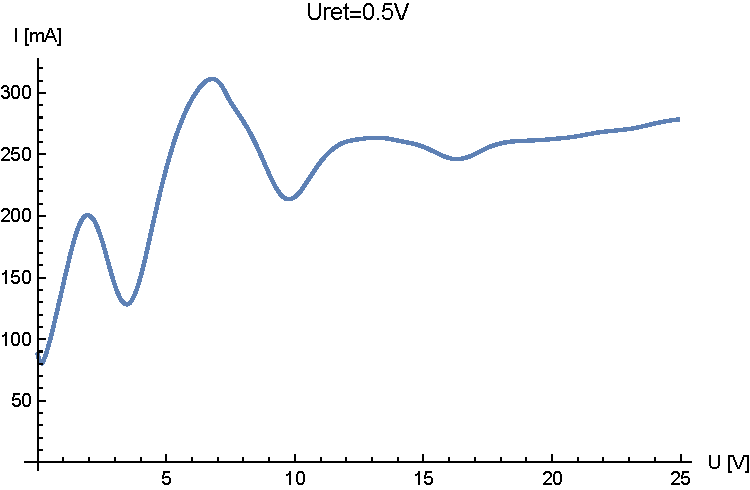
\includegraphics[width=0.625\linewidth]{wyk1}
\label{fig:wyk1}\\
\hline\\
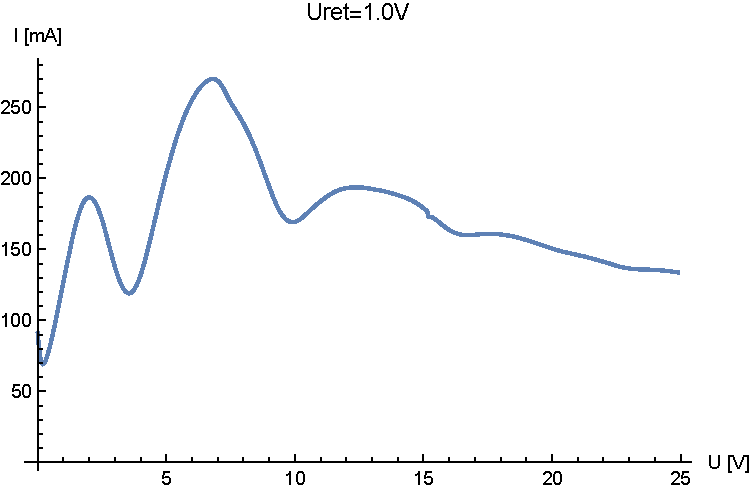
\includegraphics[width=0.625\linewidth]{wyk4}
\label{fig:wyk4}\\
\hline\\	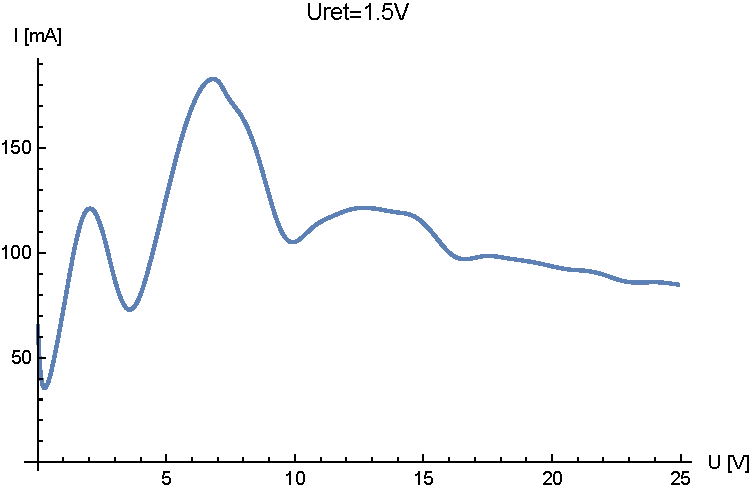
\includegraphics[width=0.625\linewidth]{wyk5}
\label{fig:wyk5}\\
\hline
\end{tabular}


\begin{tabular}{|c|}
	\hline\\
	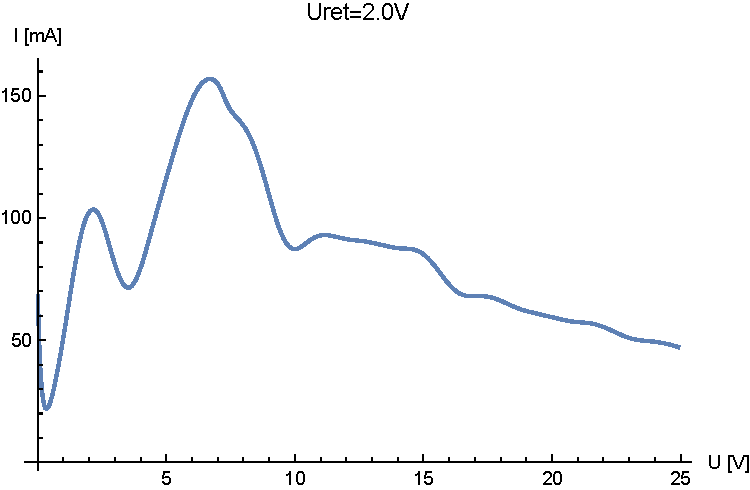
\includegraphics[width=0.6\linewidth]{wyk2}
	\label{fig:wyk2}\\
	\hline\\
	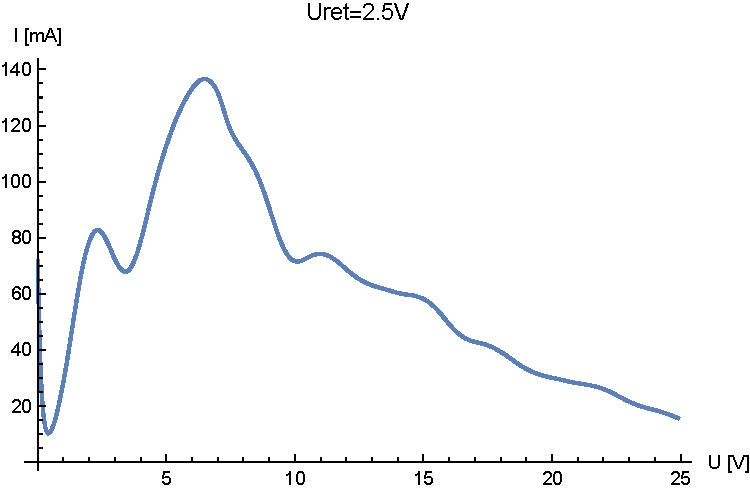
\includegraphics[width=0.6\linewidth]{wyk3}
	\label{fig:wyk3}\\
	\hline
\end{tabular}

\subsection{$T=72\:^\circ\mathrm{C}$}{
\begin{tabular}{|c|}
	\hline\\
	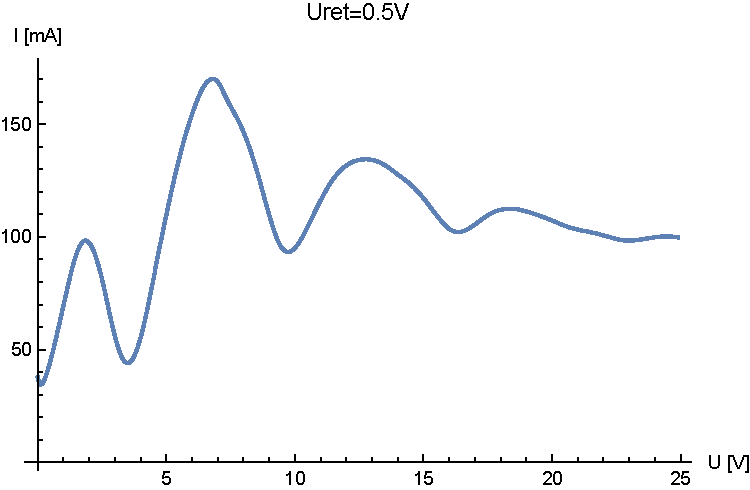
\includegraphics[width=0.6\linewidth]{wyk8}
	\label{fig:wyk8}\\
	\hline
\end{tabular}

\begin{tabular}{|c|}
	\hline\\
	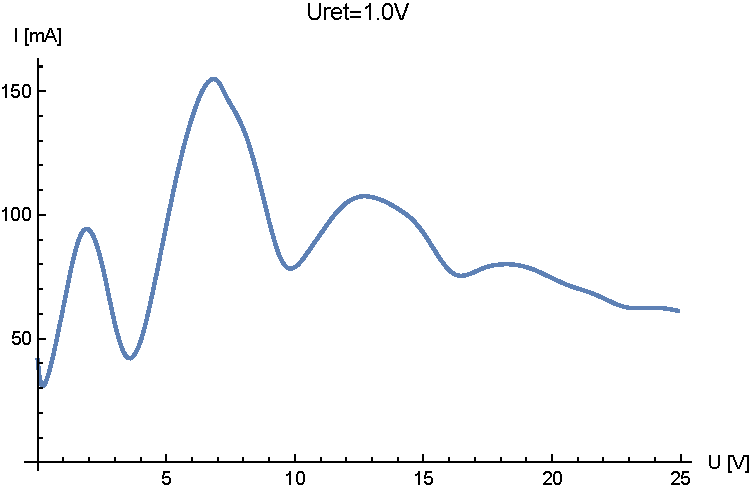
\includegraphics[width=0.7\linewidth]{wyk9}
	\label{fig:wyk9}\\
	\hline\\
	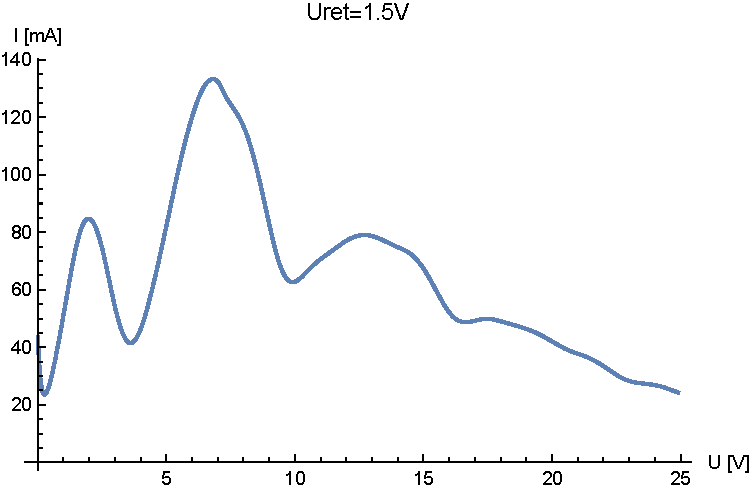
\includegraphics[width=0.7\linewidth]{wyk10}
	\label{fig:wyk10}\\
	\hline\\
	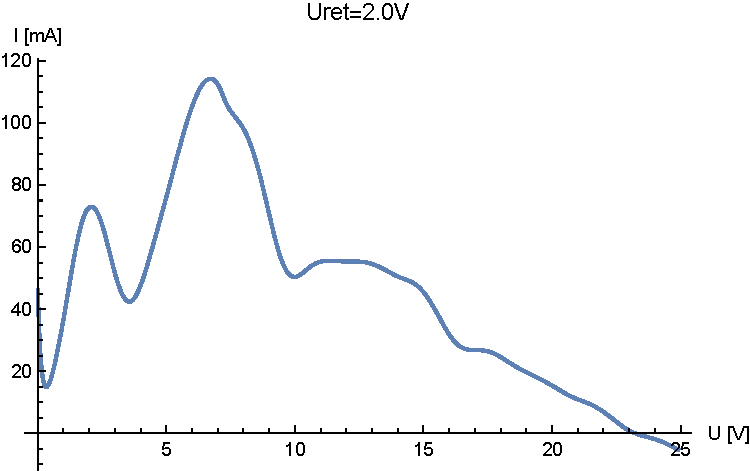
\includegraphics[width=0.7\linewidth]{wyk6}
	\label{fig:wyk6}\\
	\hline
\end{tabular}

\begin{tabular}{|c|}
	\hline\\
		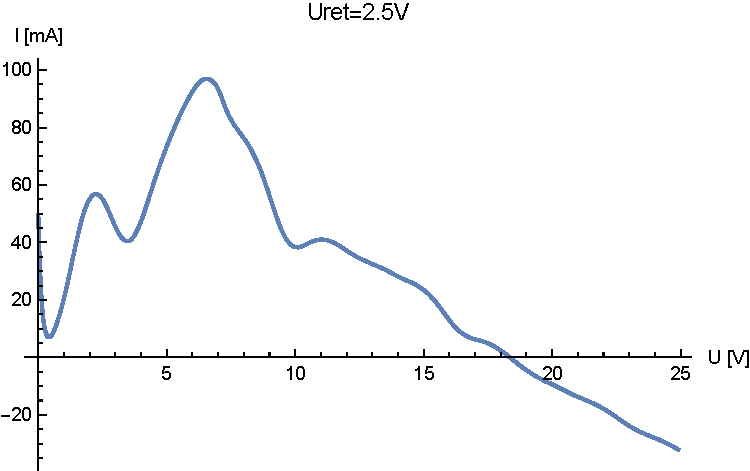
\includegraphics[width=0.65\linewidth]{wyk7}
	\label{fig:wyk7}\\
	\hline
\end{tabular}
\subsection{$T=78\:^\circ\mathrm{C}$}{

\begin{tabular}{|c|}
	\hline\\	
	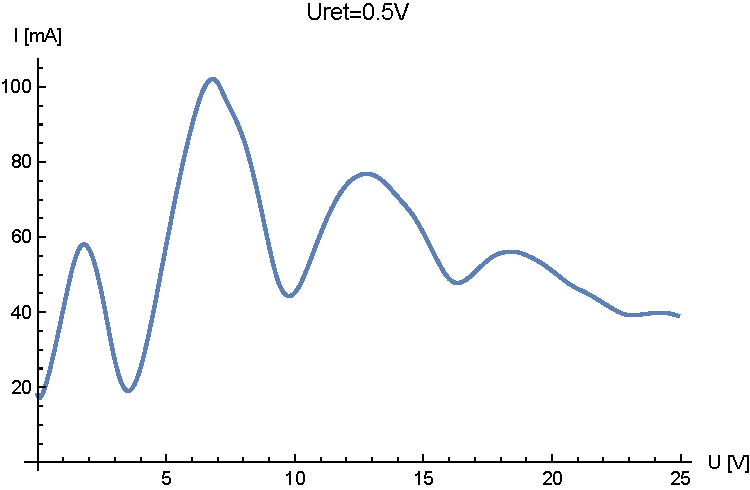
\includegraphics[width=0.625\linewidth]{wyk12}
	\label{fig:wyk12}\\
	\hline\\
	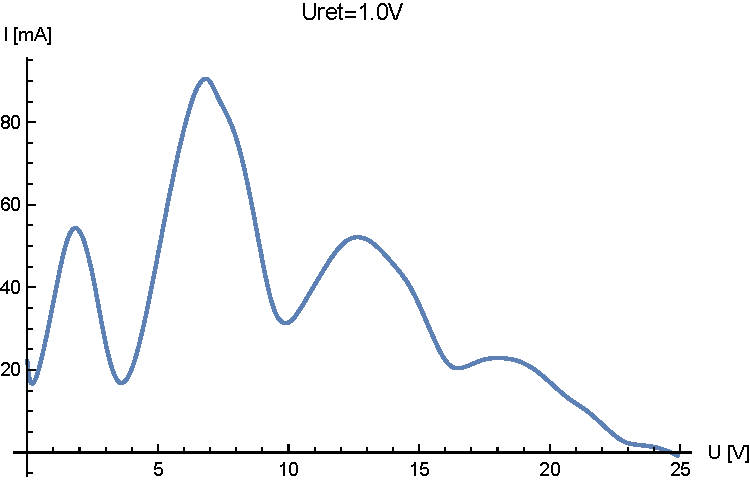
\includegraphics[width=0.625\linewidth]{wyk13}
	\label{fig:wyk13}\\
	\hline
\end{tabular}

\begin{tabular}{|c|}
	\hline\\
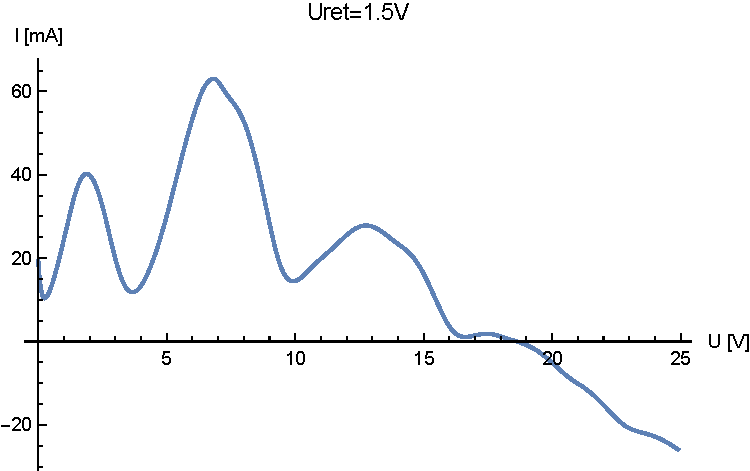
\includegraphics[width=0.7\linewidth]{wyk11}
\label{fig:wyk11}\\
\hline\\
	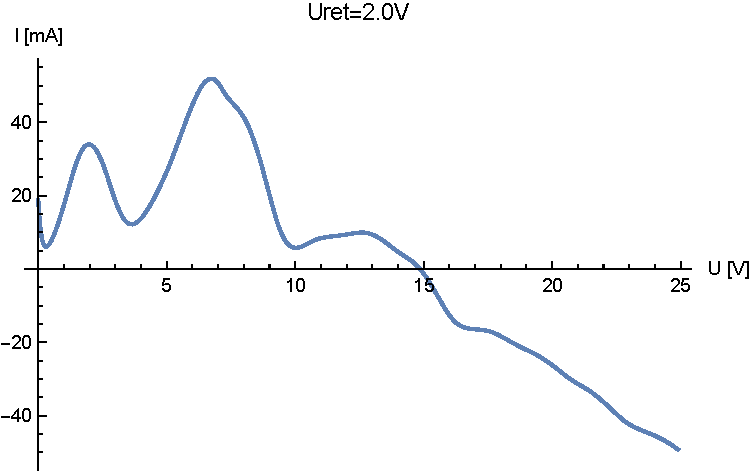
\includegraphics[width=0.7\linewidth]{wyk14}
	\label{fig:wyk14}\\
	\hline\\
	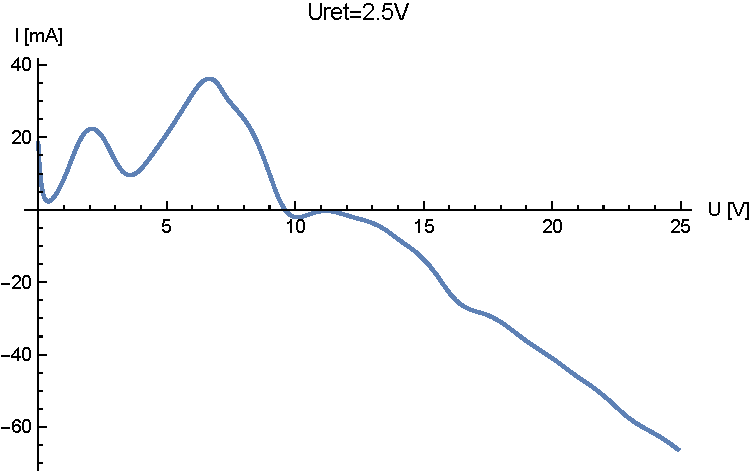
\includegraphics[width=0.7\linewidth]{wyk15}
	\label{fig:wyk15}\\
	\hline
\end{tabular}
\subsection{$T=83\:^\circ\mathrm{C}$}
\begin{tabular}{|c|}
	\hline\\
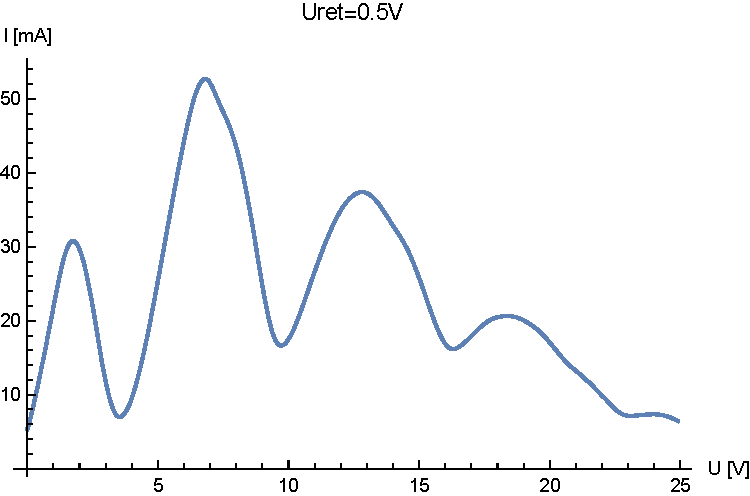
\includegraphics[width=0.625\linewidth]{wyk16}
\label{fig:wyk16}\\
\hline\\
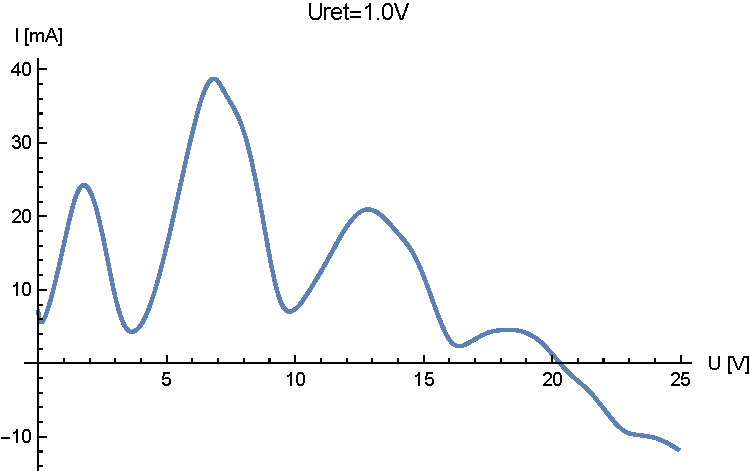
\includegraphics[width=0.625\linewidth]{wyk17}
\label{fig:wyk17}\\
\hline\\
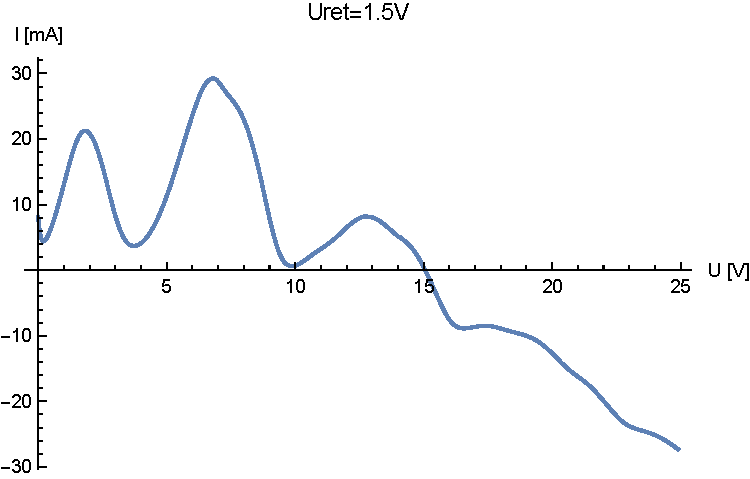
\includegraphics[width=0.625\linewidth]{wyk18}
\label{fig:wyk18}\\
\hline
\end{tabular}

\begin{tabular}{|c|}
	\hline\\
		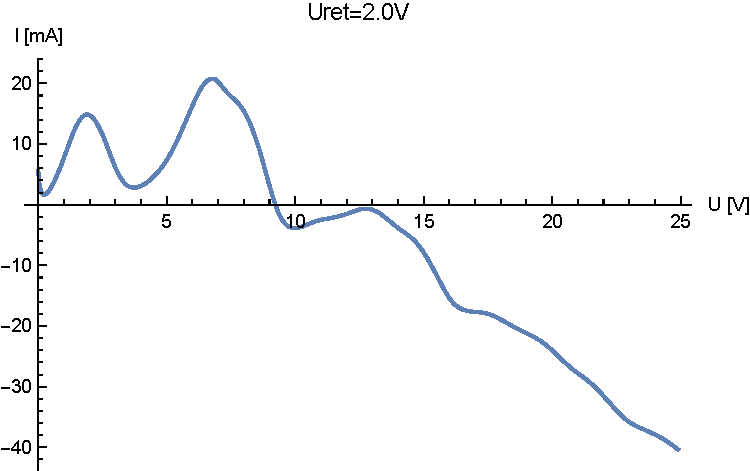
\includegraphics[width=0.8\linewidth]{wyk19}
	\label{fig:wyk19}\\
	\hline\\	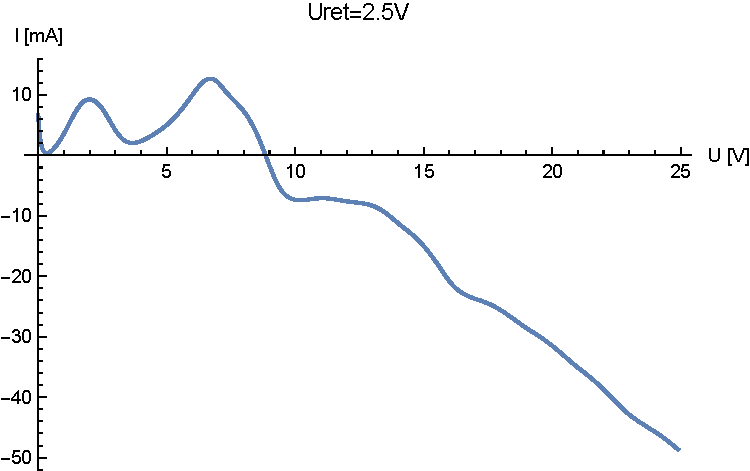
\includegraphics[width=0.8\linewidth]{wyk20}
	\label{fig:wyk20}\\
	\hline
\end{tabular}

\end{document}